\chapter{线性代数的应用}
\section{线性回归}

在前文的讨论中,我们经常面临 $A\mathbf x=\mathbf b$ 无解的问题。一个常见的例子是,一个平面内给定三个点,若这三个点不共线的话,无法解出一条直线经过这三点。但我们有“最小二乘法”,可以利用最小化损失的方式“拟合”出一条最合适的“解”。

线性代数工具可以将平面上的回归拓展到n维空间。

我们将 $\mathbf b$ 分解,一部分为 $\mathbf b$ 向 $A$ 的列空间的投影 $\mathbf p$,另一部分为 $\mathbf e$ 。显然有 $\mathbf e=\mathbf b-\mathbf p$ 。$A\mathbf x=\mathbf b$ 无解,但是 $A\hat{\mathbf{x}}=\mathbf p$ 有解。

将向量的模长平方可以得到
$$
||A\mathbf x-\mathbf b||^2=||A\mathbf x-\mathbf p||^2+||\mathbf e||^2
$$

\begin{figure}
	\centering
	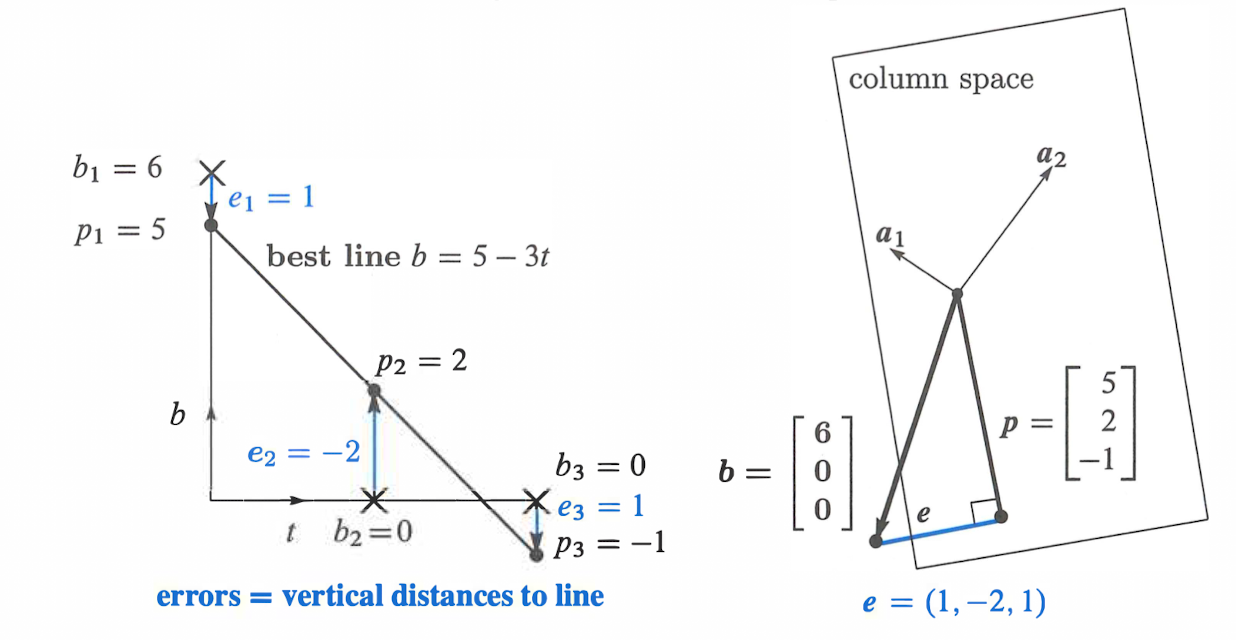
\includegraphics[width=0.7\linewidth]{../img/screenshot003}
	\caption{线性回归问题的两种表述方式}
	\label{image_linead_approx}
\end{figure}

由图\ref{image_linead_approx},可以看出 $\mathbf b$ 不在空间 $A$ 中,这也是为什么 $A\mathbf x =\mathbf b$ 无解。但我们可以通过投影实现最小化 $\mathbf e=\mathbf b-A\hat{\mathbf x}$ 。

我们也可以对 $\text E=||A\mathbf x -\mathbf b||$ 求偏导,使偏导值为零,可以得到当 $A^\top A\hat{\mathbf x}=A^\top\mathbf b$ 偏导值为 $\mathbf 0$ 。我们发现,这个结果与投影形式是一致的。

至此, $\hat x$ 就是我们想要得到的结果
$$
\hat x=(A^\top A)^{-1}A^\top\mathbf b
$$

读者可以尝试在二维条件下验证一下这个公式是否与最小二乘法公式吻合。

\section{坐标变换}

坐标变换是工程中非常常用的操作,对于两个坐标系之间的变换,我们可以拆分为旋转和平移两个操作。

如下操作,我们实现了将坐标 $\mathbf v$ 转换到 $\mathbf u$ 
$$
\mathbf u =R\mathbf v+\mathbf t
$$
其中, $R$ 是前文所提到过的旋转矩阵, $\mathbf t$ 为前文提到的平移向量。

通常我们用增广矩阵的工具,使这个式子更加简结
$$
\begin{bmatrix}
\mathbf u\\1
\end{bmatrix}=
\begin{bmatrix}
	R & \mathbf t
\end{bmatrix}
\begin{bmatrix}
	\mathbf v\\1
\end{bmatrix}
$$

\section{概率论}

首先介绍一下概率论中我们的几个基本概念。

\begin{itemize}
	\item \textbf{期望}: $\mathbf{E}[\mathbf x]=\sum_{i=1}^np_ix_i$
	\item \textbf{样本方差}: $\mathbf S[\mathbf x]=\frac{1}{n-1}\sum_{i=1}^n(x_i-m)^2$ ,其中 $m$ 是样本的平均值。
	\item \textbf{方差}: $\sigma^2=\mathbf E[(\mathbf x-m)^2]=\sum_{i=1}^np_i(x_i-m)^2$
	\item \textbf{协方差}: $\mathbf E[(X-\mathbf E X)(Y -\mathbf E Y)]$
\end{itemize}

协方差可能会是一个较陌生的概念,从直观上来看,协方差表示的是两个变量总体误差的期望。我们可以用协方差来表示两个变量之间的相关性。协方差为0的两个随机变量称为是不相关的。

当变量多于两个时,我们计算变量间的协方差可以借助线性代数进行。

$$
\mathbf S=\mathbf E[(\mathbf X-\mathbf E \mathbf X)(\mathbf X -\mathbf E \mathbf X)^\top]
$$

我们就称 $\mathbf S$ 为\textbf{协方差矩阵}。

还是以二维的两个随机变量 $X,Y$ 为例
$$
\begin{aligned}
	\mathbf S&=\mathbf E[\begin{bmatrix}X-\mathbf E X\\Y-\mathbf E Y\end{bmatrix}
	\begin{bmatrix}X-\mathbf E X&Y-\mathbf E Y\end{bmatrix}]\\&=
	\begin{bmatrix}
		\mathbf E(X-\mathbf E X)(X-\mathbf E X)&\mathbf E(X-\mathbf E X)(Y-\mathbf E Y)\\
		\mathbf E(Y-\mathbf E Y)(X-\mathbf E X)&\mathbf E(Y-\mathbf E Y)(Y-\mathbf E Y)\\
	\end{bmatrix}
\end{aligned}
$$
可以看出,协方差矩阵是一个对称矩阵,对角线上是所有变量的方差,其余位置为两两的协方差。通过协方差矩阵,我们可以很轻松地显示出变量之间的相关性。